%File: adc_aware_llm_aaai2027.tex
%AAAI 2027 anonymous submission -- main paper.
%Supplementary material: adc_aware_llm_aaai2027_supplementary.tex
\documentclass[letterpaper]{article} % DO NOT CHANGE THIS
\usepackage[submission]{aaai2027}  % DO NOT CHANGE THIS
\usepackage[hyphens]{url}  % DO NOT CHANGE THIS
\usepackage{graphicx} % DO NOT CHANGE THIS
\urlstyle{rm} % DO NOT CHANGE THIS
\def\UrlFont{\rm}  % DO NOT CHANGE THIS
\usepackage{natbib}  % DO NOT CHANGE THIS AND DO NOT ADD ANY OPTIONS TO IT
\usepackage{caption} % DO NOT CHANGE THIS AND DO NOT ADD ANY OPTIONS TO IT
\frenchspacing  % DO NOT CHANGE THIS
%
\usepackage{amsmath}
\usepackage{amssymb}
\usepackage{amsthm}
\usepackage{booktabs}
\usepackage{multirow}
%
\usepackage{tikz}
\usetikzlibrary{arrows.meta,positioning,calc}
\definecolor{myblue}{HTML}{2E86AB}
\definecolor{myorange}{HTML}{E07A5F}
\definecolor{mygray}{HTML}{AAAAAA}
\definecolor{mybluedark}{HTML}{1A5276}
%
\usepackage{algorithm}
\usepackage{algorithmic}
%
\DeclareCaptionStyle{ruled}{labelfont=normalfont,labelsep=colon,strut=off} % DO NOT CHANGE THIS
%
\theoremstyle{plain}
\newtheorem{lemma}{Lemma}
\newtheorem{corollary}{Corollary}
%
% Placeholder for in-progress multi-model runs. Every row that uses it ends
% with a "% TODO(<model>): ..." comment. Inventory: grep -n 'phnum\|TODO(' *.tex
\newcommand{\phnum}{XX.X}
%
\pdfinfo{
/TemplateVersion (2027.1)
}

\setcounter{secnumdepth}{0}

\title{ADC-Aware Post-Training Adaptation for Analog LLM Inference under Fixed Output Quantization}
\author{Anonymous Submission}
\affiliations{}

\begin{document}

\maketitle

\begin{abstract}
Analog in-memory and optical accelerators promise energy-efficient inference for large language models (LLMs), but every analog matrix--vector product must pass through a finite-resolution analog-to-digital converter (ADC) whose step size is fixed in hardware. Existing methods do not fit this constraint: standard LLM quantization optimizes only the input-side weight and activation quantizers and leaves the output lattice unmodeled, while analog-aware approaches rely on hardware-in-the-loop retraining that is prohibitively expensive at LLM scale and must be repeated per model and configuration. We present the first fully post-training alternative: ADC-aware calibration reshapes what enters the converter, and a lightweight residual correction ($0.23\%$ extra parameters), placed \emph{after} the converter---where the information is actually lost---recovers what calibration cannot. On Llama-3.2-1B, a naive W4A4 analog model collapses to 2354.86 WikiText-2 perplexity; our pipeline restores 14.03 (23.20 on C4), surpassing an INT8 analog PTQ baseline at a quarter of its bit-width. We evaluate on four sub-2B open LLMs, and the recipe transfers unchanged to a hardware-realistic unsigned shift-subtract readout.
\end{abstract}

\section{Introduction}

LLM inference is dominated by dense linear projections, and autoregressive decoding is memory-bandwidth-bound: each generated token reads billions of parameters to produce a single output, so throughput is limited by data movement rather than arithmetic \citep{pope2023efficiently}. In-memory computing (IMC) and optical accelerators attack this bottleneck by executing matrix--vector multiplication (MVM) directly in the physical substrate that stores the weights \citep{xiao2021accuracy,legallo2023mixed,spall2022hybrid}. The analog array performs the accumulation---but the next transformer operation still expects a digital tensor, so every analog MVM is followed by an analog-to-digital converter on the inference path.

That readout stage is the central object of this paper. In a purely digital low-bit model, the dominant approximation error comes from quantizing weights and activations, and the corresponding step sizes are free calibration variables. The ADC adds an output-side quantizer of a different kind: after each analog accumulation it floors the result onto a uniform lattice whose step $\Delta$ is set by tile width, ADC precision, and range scaling---all fixed at hardware design time. Calibration can reshape the signal that enters the converter, but it cannot make the lattice finer. Even perfectly quantized weights and activations can therefore be accumulated into values that are rounded coarsely, clipped at the ADC range, or collapsed into a dead zone around zero (Figure~\ref{fig:deadzone}).

\begin{figure*}[t]
\centering
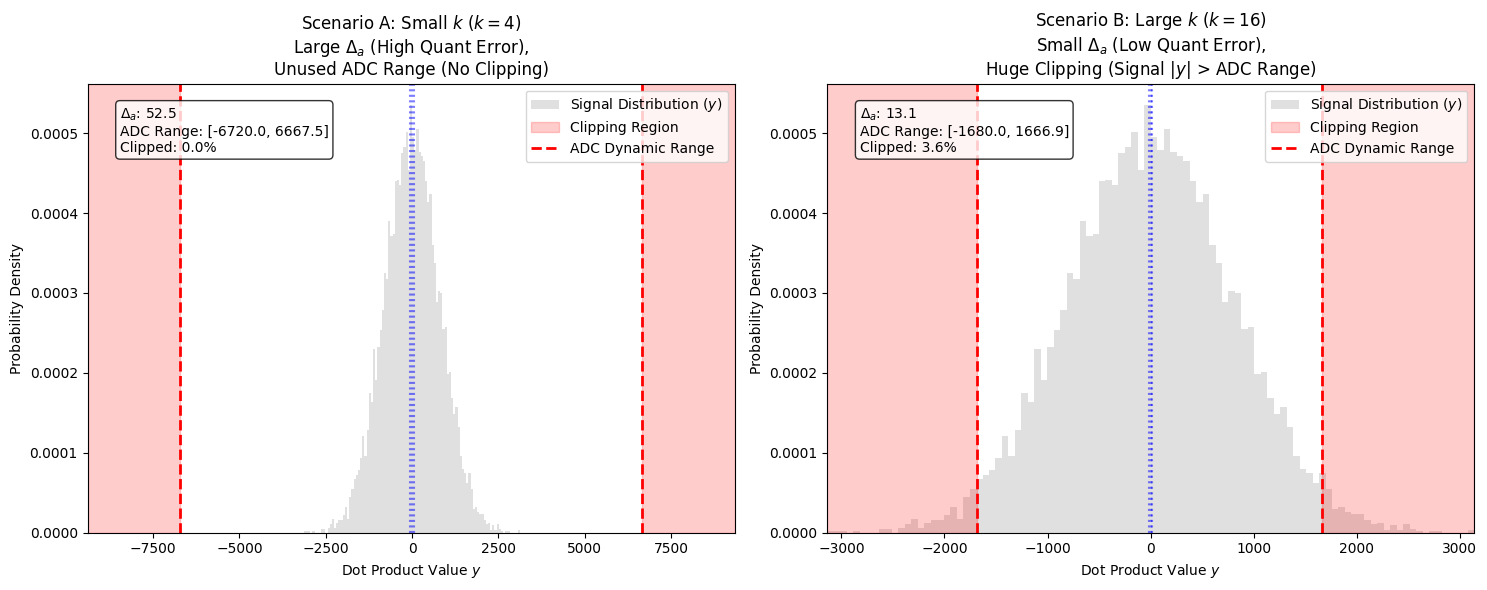
\includegraphics[width=0.74\textwidth]{figs/dead_zone.png}
\caption{The ADC range--resolution tradeoff set by the fixed scaling factor $k$ (and hence $\Delta$). Small $k$ (left) gives a large step $\Delta$: the accumulation distribution fits inside the ADC range with no clipping, but the lattice is coarse. Large $k$ (right) shrinks $\Delta$ for finer resolution, yet the tails of the distribution now exceed the ADC range and are clipped. Because $k$ is fixed in hardware, calibration alone cannot escape this tradeoff.}
\label{fig:deadzone}
\end{figure*}

LLMs are a worst case for this failure mode. Transformer hidden states contain rare but very large outlier channels \citep{dettmers2022llmint8,xiao2022smoothquant}. Under per-token max scaling, a single outlier channel determines the activation scale and compresses typical channels into a narrow band of small integer codes. Accumulated tile by tile and passed through the coarse ADC lattice, those codes occupy few output bins, and small accumulations collapse to zero. Standard LLM PTQ reduces input-side quantization error, but it never optimizes the post-accumulation ADC output.

Existing analog-aware remedies such as RAOQ \citep{tang2024raoq} and Analog Foundation Models \citep{buchel2025analog} confirm that this output-side bottleneck is real, but they close it with quantization-aware training or hardware-aware finetuning: end-to-end gradient training of the full model with the hardware in the loop, repeated for every model and hardware configuration. Our question is narrower and, we argue, more deployment-relevant: starting from a pretrained decoder-only LLM, how far can \emph{post-training} adaptation alone go?

Our answer is a fully post-training, \emph{two-phase} pipeline organized around the analog--digital boundary. Phase~1 performs ADC-aware PTQ calibration \emph{before} the converter, reducing how much information the fixed lattice destroys. Phase~2 attaches a lightweight residual correction \emph{after} the converter, compensating in the digital domain for the information the lattice still destroys. This separation between pre-ADC calibration and post-ADC correction is the key conceptual distinction of the method.

We evaluate the pipeline on four sub-2B open-weight models---Llama-3.2-1B, Qwen2.5-1.5B, OLMo-1B, and TinyLlama-1.1B---under a tiled analog simulator with an 8-bit ADC. Our contributions are as follows. \textbf{First}, we formulate decoder-only LLM inference under a tiled ADC-constrained MVM model and isolate ADC-induced error from ordinary quantization error using bypass evaluation and per-layer diagnostics (dead-rate, clip-rate, bin usage). \textbf{Second}, we develop an ADC-aware PTQ recipe---cross-block propagation of ADC-corrupted hidden states, an $\alpha$-mixed clean/ADC objective, and bounded per-channel diagonal scaling under a staged schedule---backed by a lemma showing that orthogonal Kronecker transforms have an intrinsic ceiling on outlier suppression. On Llama-3.2-1B this turns a collapsed naive W4A4 baseline (WikiText-2 perplexity 2354.86) into a usable model (26.66). \textbf{Third}, we introduce a post-ADC rank-4 residual LoRA correction that trains only $0.23\%$ additional parameters against a frozen analog path, reduces WikiText-2/C4 ADC perplexity to 14.03/23.20, and surpasses our INT8 ADC PTQ baseline (Table~\ref{tab:main}). \textbf{Finally}, we show that the recipe transfers to a hardware-realistic unsigned shift-subtract readout, where per-layer ADC range search and post-ADC correction are complementary.

\section{Background and Related Work}

\subsection{ADC-Constrained Analog Inference}

Analog in-memory and optical accelerators reduce data movement by executing MVM directly in the substrate that stores the weights \citep{xiao2021accuracy,spall2022hybrid,legallo2023mixed}: weights map to physical states, the input is applied as an analog excitation, and array physics performs the accumulation. The result is analog while the next transformer operation expects a digital tensor, so each MVM is followed by an ADC---an output quantizer applied \emph{after} accumulation, with a step size fixed by hardware. It is therefore a distinct error source, not an implementation detail.

Recent analog-aware methods make this point explicit. RAOQ addresses output quantization through a dedicated training stage after QAT \citep{tang2024raoq}, and Analog Foundation Models adapts pretrained LLMs to noisy low-precision analog hardware with a broader hardware-aware training pipeline \citep{buchel2025analog}. Such end-to-end training scales poorly to the LLM regime: it needs full-precision gradients through every quantized layer and must be repeated per model and per hardware configuration. We build on the same diagnosis---ADC output quantization is a first-class bottleneck---but pursue a strictly post-training regime.

\subsection{Low-Bit LLM Quantization}

Quantization maps real-valued tensors to low-bit integer codes to cut memory, bandwidth, and arithmetic cost \citep{gholami2021survey,jacob2018quantization}; PTQ calibrates scales and transforms on a small dataset, while QAT places quantization inside the training loop with straight-through estimators (STE) for the non-differentiable rounding \citep{esser2019learned}. LLMs are hard to quantize because their hidden states are anisotropic and outlier-heavy. SmoothQuant migrates dynamic range from activations into weights \citep{xiao2022smoothquant}; Outlier Suppression+ adds channel-wise shifting and scaling \citep{wei2023outlier}; AWQ protects salient weights \citep{lin2023awq}; OmniQuant combines learnable clipping with equivalent transformations \citep{shao2023omniquant}; GPTQ frames weight quantization as second-order reconstruction \citep{frantar2022gptq}. Rotation-based QuaRot and SpinQuant suppress residual-stream outliers with fixed or learned rotations \citep{ashkboos2024quarot,liu2024spinquant}, while FlatQuant learns invertible per-projection Kronecker transforms and folds them into the weights \citep{liu2024flatquant}. CBQ and quantization-error-propagation PTQ model how error accumulates across depth \citep{ding2023cbq,qep2025}. All of these optimize the \emph{input side}: even when error propagation is included, the target remains a digital hidden-state reconstruction. None models the separate, hardware-fixed output lattice of an ADC.

\subsection{Lightweight Post-Quantization Adaptation}

When pure PTQ saturates, a natural next step is to freeze the quantized backbone and attach a small trainable correction. Aggressively quantized transformers often benefit from finetuning or QAT-style recovery \citep{liu2023llmqat,chen2024efficientqat}, and low-rank methods such as LoRA and quantization-error reconstruction capture much of the residual error with few trainable parameters \citep{hu2022lora,zhang2024lqer}.

For ADC-constrained inference this family is particularly attractive: a frozen quantized analog path preserves the hardware mapping while a small digital branch learns the remaining distortion. What is non-standard in our setting is the \emph{placement} of the correction---not before quantization, but after the ADC, on the digital side of the analog--digital boundary. The gap we target is thus twofold: existing PTQ optimizes input-side error while the ADC imposes a distinct output-side bottleneck that must be modeled explicitly; and once transform-based PTQ saturates, it has been unclear where a lightweight correction should be inserted and how it should be trained. We address both within a fully post-training budget.

\section{Problem Statement}

\begin{figure}[t]
\centering
\resizebox{\linewidth}{!}{%
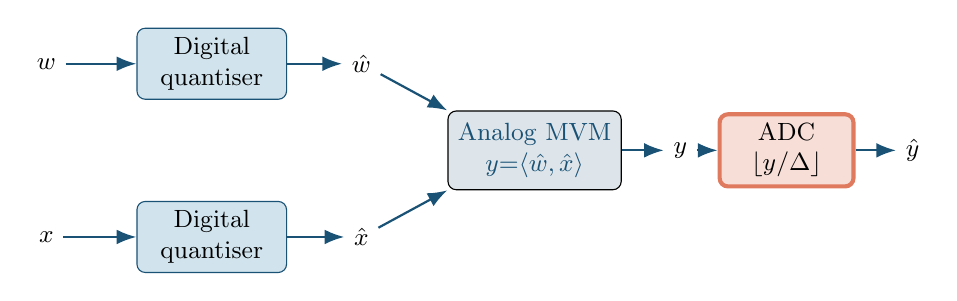
\begin{tikzpicture}[
    every node/.style={font=\small},
    q/.style={draw=mybluedark, rounded corners=3pt, fill=myblue!22,
              minimum width=1.9cm, minimum height=0.72cm, align=center},
    tile/.style={draw, rounded corners=3pt, fill=mybluedark!15, text=mybluedark,
                 minimum width=2.2cm, minimum height=1.0cm, align=center},
    adc/.style={draw=myorange, line width=1.5pt, rounded corners=3pt,
                fill=myorange!25, minimum width=1.7cm, minimum height=0.72cm,
                align=center},
    arr/.style={-{Latex[length=2.5mm]}, thick, mybluedark}
  ]
  \node (w)  at (0,   1.1) {$w$};
  \node[q] (qw) at (2.1,  1.1) {Digital\\quantiser};
  \node (wb) at (4.0,  1.1) {$\hat w$};
  \node (x)  at (0,  -1.1) {$x$};
  \node[q] (qx) at (2.1, -1.1) {Digital\\quantiser};
  \node (xb) at (4.0, -1.1) {$\hat x$};
  \draw[arr] (w)--(qw);   \draw[arr] (qw)--(wb);
  \draw[arr] (x)--(qx);   \draw[arr] (qx)--(xb);
  \node[tile] (T) at (6.2, 0) {Analog MVM\\$y{=}\langle\hat w,\hat x\rangle$};
  \draw[arr] (wb) -- (T.north west);
  \draw[arr] (xb) -- (T.south west);
  \node (y)  at (8.05, 0) {$y$};
  \draw[arr] (T)--(y);
  \node[adc] (A) at (9.4, 0) {ADC\\$\lfloor y/\Delta\rfloor$};
  \draw[arr] (y)--(A);
  \node (yb) at (11.0, 0) {$\hat y$};
  \draw[arr] (A)--(yb);
\end{tikzpicture}}
\caption{Math model of an analog linear layer. Weights $w$ and activations $x$ are digitally quantized to $\hat w,\hat x$, multiplied in the analog matrix--vector unit, and the accumulation $y$ is mapped back to the digital domain by a fixed-resolution ADC, $\hat y = \Delta\lfloor y/\Delta\rfloor$. The output-side ADC step is set by hardware and is not a free calibration variable.}
\label{fig:optical}
\end{figure}

We consider a pretrained decoder-only transformer whose linear projections $y = xW^{\top} + b$ execute on a tiled ADC-constrained accelerator (Figure~\ref{fig:optical}). The contraction dimension is split into tiles of width $M$. For tile $t$, activations are quantized per token and weights per output channel,
\begin{equation}
    x_t \approx s_{x,t}\,\hat{x}_t,
    \qquad
    W_t \approx \operatorname{diag}(\mathbf{s}_{w,t})\,\hat{W}_t,
    \label{eq:codes}
\end{equation}
and the analog array accumulates the integer dot product $z_t = \hat{x}_t \hat{W}_t^{\top}$. Unlike in digital inference, $z_t$ is not available at full precision: the ADC discretizes each tile output,
\begin{equation}
    Q_{\mathrm{ADC}}(z_t;\Delta,n_a,p_a)
    = \Delta\cdot\operatorname{clip}\!\left(\left\lfloor \tfrac{z_t}{\Delta} \right\rfloor,\, n_a,\, p_a\right),
    \label{eq:adc}
\end{equation}
with code bounds $(n_a,p_a)$, and the projection output is reassembled digitally,
\begin{equation}
    \hat{y} = b + \sum_t s_{x,t}\left(\mathbf{s}_{w,t} \odot Q_{\mathrm{ADC}}(z_t;\Delta,n_a,p_a)\right).
    \label{eq:dequant}
\end{equation}

The step $\Delta$ is a hardware constant. For the signed (bipolar) readout used in our main experiments,
\begin{equation}
    \Delta = \frac{2\,M\,q_x\,q_w}{2^{b_a}\,k},
    \label{eq:delta}
\end{equation}
where $b_a$ is the ADC bit-width, $k$ the range-scaling factor, and $q_x,q_w$ the maximum activation and weight code levels set by the precisions $b_x,b_w$. For the unsigned shift-subtract readout evaluated later,
\begin{equation}
    \Delta_u = \frac{M\,(2^{b_x}-1)(2^{b_w}-1)}{2^{b_a}\,k}.
    \label{eq:delta_u}
\end{equation}
In both cases the essential property is the same: every term is fixed by hardware, so the output lattice cannot be made finer by calibration. If $0 \le z_t < \Delta$, the tile output collapses to the zero code (a \emph{dead zone}); if $z_t$ exceeds the ADC range, it is clipped.

The software-side degrees of freedom are transform-based PTQ parameters $\phi$ and, in the second phase, a small residual branch $\psi$. Following FlatQuant, an invertible transform can be inserted into a projection without changing the full-precision map, $xW^{\top} = (xT^{-1})(TW^{\top})$; after quantization and ADC discretization this equivalence no longer holds exactly, so calibration chooses $\phi$ to minimize the block-level mismatch
\begin{equation}
    \min_{\phi}\;
    \mathbb{E}_{x \in \mathcal{C}}
    \left[\left\| B_\ell(x) - \hat{B}^{\mathrm{ADC}}_\ell(x;\phi,\mathcal{H}) \right\|_2^2\right],
    \label{eq:calib}
\end{equation}
where $B_\ell$ is the full-precision block, $\hat{B}^{\mathrm{ADC}}_\ell$ its ADC-constrained counterpart, $\mathcal{C}$ a small calibration set, and $\mathcal{H} = (b_x, b_w, b_a, M, k, \mathrm{readout})$ the fixed hardware tuple. At the model level, the goal is to minimize perplexity under fixed $\mathcal{H}$ with $|\psi| \ll |\theta|$, where $\psi = 0$ recovers pure PTQ.

The study is organized around five research questions: \textbf{(RQ1)} how much degradation is caused specifically by ADC output quantization; \textbf{(RQ2)} to what extent transform-based PTQ can mitigate it; \textbf{(RQ3)} whether reconstruction-only calibration suffices, or explicitly ADC-aware objectives are required; \textbf{(RQ4)} which layers and projections are most ADC-sensitive; and \textbf{(RQ5)} when adaptation beyond pure PTQ becomes necessary. The experiments answer these questions in turn, and the conclusion returns to them explicitly. Throughout, hardware behavior is studied with a software simulator that models tiled integer MVM, per-token/per-channel quantization, ADC floor and clipping, and dequantization, while abstracting device-level non-idealities such as noise, drift, and IR drop.

\section{ADC-Aware Post-Training Adaptation}

Our pipeline is \emph{two-phase}. Phase~1 is ADC-aware PTQ calibration: it learns per-projection transforms and scalings that reshape what enters the converter. Phase~2 is post-ADC residual correction: it attaches a small digital branch after the converter and trains it with the analog path frozen. Within Phase~1, the calibration schedule itself is split into \emph{Stage~A} and \emph{Stage~B}; throughout the paper, ``Stage'' refers exclusively to this schedule, never to the two phases of the pipeline.

\subsection{Phase 1 Baseline: FlatQuant}

FlatQuant exploits a linear invariance of the MVM. For any invertible $T$,
\begin{equation}
    y = xW^{\top} = (xT^{-1})(TW^{\top}),
    \label{eq:flatquant}
\end{equation}
so choosing $T$ to flatten the distribution of $xT^{-1}$ improves both integer quantization and ADC bin coverage while preserving the map. A full $d\times d$ transform is prohibitive, so FlatQuant parameterizes $T = T_1 \otimes T_2$, reducing the trainable parameters from $\mathcal{O}(d^2)$ to $\mathcal{O}(d)$ \citep{liu2024flatquant}. We wrap all seven projections of each decoder block ($q,k,v,o$ in attention and \texttt{gate}, \texttt{up}, \texttt{down} in the FFN).

Calibration is teacher--student: a frozen FP teacher produces the target and the quantized student minimizes the reconstruction error over the Kronecker factors; after calibration, $T$ folds into the weights at no inference cost. Standard block calibration uses clean teacher activations,
\begin{equation}
    \mathcal{L}_{\mathrm{FP}} = \left\| \hat{B}(x^{\star}) - B_{\mathrm{FP}}(x^{\star}) \right\|_2^2,
    \label{eq:lfp}
\end{equation}
which is well matched to digital PTQ but mismatched to analog deployment, where each block receives activations already corrupted by prior ADC readouts.

\subsection{Cross-Block Propagation and $\alpha$-Mixing}

To match deployment, blocks are calibrated sequentially from layer $0$ to $L-1$. When calibrating block $\ell$, its input is the ADC-quantized output of the already calibrated block $\ell-1$, so the block sees during calibration the same accumulated distortion it will see at inference:
\begin{equation}
    \mathcal{L}_{\mathrm{ADC}} = \left\| \hat{B}(\hat{x}) - B_{\mathrm{FP}}(x^{\star}) \right\|_2^2,
    \label{eq:ladc}
\end{equation}
where $\hat{x}$ is the ADC-propagated hidden state. Full propagation is noisy in W4A4 because gradients must pass through several floor operators via STE. We therefore interpolate between the clean and propagated objectives,
\begin{equation}
    \mathcal{L}(\alpha) = (1-\alpha)\,\mathcal{L}_{\mathrm{FP}} + \alpha\,\mathcal{L}_{\mathrm{ADC}}.
    \label{eq:alpha}
\end{equation}
The clean term stabilizes the transform; the propagated term teaches robustness to ADC distortion. A sweep (Appendix~C of the supplementary material) shows that $\alpha = 0.5$ is the best W4A4 point: below it the ADC regime is under-weighted, above it floor-induced gradient noise degrades transform quality. At INT8, propagation alone drops ADC perplexity from $28.86$ to $14.55$ with no extra parameters.

\subsection{Bounded Per-Channel Diagonals}

Propagation and $\alpha$-mixing fix \emph{what} the calibration optimizes, but the transform family still has limited capacity to tame outliers: rotations redistribute energy across channels without rescaling any of them. We first make this precise.

\begin{lemma}[Rotation-only outlier suppression bound]
\label{lem:rotation}
Let $P = L \otimes R$ with $L^\top L = I$, $R^\top R = I$ be an orthogonal Kronecker transform on $\mathbb{R}^d$, and define the effective participation ratio $m_{\mathrm{eff}}(x) = \|x\|_2^2 / \|x\|_\infty^2 \in [1, d]$. Then for every such $P$,
\begin{equation}
    \|xP\|_\infty \;\ge\; \frac{\|x\|_2}{\sqrt{d}},\qquad
    \frac{\|x\|_\infty}{\min_{P}\|xP\|_\infty} \;\le\; \sqrt{\frac{d}{m_{\mathrm{eff}}(x)}} .
\end{equation}
\end{lemma}

The proof (Appendix~B of the supplementary material) follows from orthogonal invariance of $\|\cdot\|_2$ and the $\ell^\infty$--$\ell^2$ inequality. With $d = 2048$ and $8$ dominant channels ($m_{\mathrm{eff}} \approx 8$), the peak can be suppressed by at most a factor of $16$; the Kronecker family is moreover a strict low-dimensional subset of all orthogonal transforms, so the reachable suppression can be smaller still. If more suppression is required, rotation alone is provably insufficient.

We therefore absorb a trainable diagonal $D = \mathrm{diag}(d_1,\ldots,d_c)$, $d_i \in [10^{-4}, 10]$, into the transform, preserving the map by equal-and-opposite rescaling of the weights,
\begin{equation}
    y = (x\,D^{-1}T^{-1})(T\,D\,W^{\top}).
    \label{eq:diag}
\end{equation}
Because $D$ is not orthogonal, it escapes the $\ell^2$-energy invariance behind Lemma~\ref{lem:rotation}: setting $d_j < 1$ shrinks an outlier channel \emph{before} the per-token scale is computed, achieving suppression no rotation can match, while the box bounds prevent degenerate scaling. $D$ folds into the weights at deployment. We place separate diagonals on the attention path and the MLP path; ablations show they play different roles---MLP diagonals drive no-ADC transform quality, attention diagonals close the ADC gap.

\subsection{Staged Calibration}

With the objective and transform family in place, the last question is how to optimize them together. Training all Kronecker factors and both diagonals jointly at $\alpha = 0.5$ is unstable: attention gradients dominate before the MLP transforms converge. We therefore split calibration into two stages. \emph{Stage~A} trains the MLP Kronecker factors and MLP diagonals with clean reconstruction ($\alpha = 0$), giving a stable warm start. \emph{Stage~B} freezes the MLP diagonals, unfreezes the attention factors and attention diagonals, and fine-tunes with $\mathcal{L}(0.5)$ at a $10\times$ lower learning rate. This schedule avoids gradient interference and yields the best pure-PTQ checkpoint (bypass $18.50$, ADC $27.60$ on Llama-3.2-1B). Algorithm~\ref{alg:calibration} makes the procedure precise; gradients through $Q_x,Q_w,Q_{\mathrm{ADC}}$ use STE.

\begin{algorithm}[tb]
\caption{ADC-Aware Staged PTQ Calibration (Phase 1)}
\label{alg:calibration}
\textbf{Input}: FP model $F$ with teacher blocks $\{B^{\mathrm{FP}}_\ell\}_{\ell=1}^{L}$; calibration set $C$; hardware $\mathcal{H}=(M,b_a,k,q_x,q_w)$ fixing $\Delta$; base lr $\eta$; epochs $E_A,E_B$; box $[\underline{d},\overline{d}]=[10^{-4},10]$\\
\textbf{Output}: Quantized ADC-aware model $\hat{F}_{\mathrm{ADC}}$
\begin{algorithmic}[1]
\STATE \textbf{Def.} $\tilde{T}_p:=T_pD_p$; per projection $p$,\\
\quad $\hat{f}_p(x)=D_{\mathrm{out}}Q_{\mathrm{ADC}}\!\big(Q_w(\tilde{T}_pW_p^\top)\,Q_x(x\tilde{T}_p^{-1})\big)$; \\
\quad $\hat{B}_\ell(\cdot;\theta)$ composes $\{\hat{f}_p\}$ over $p\in\mathcal{P}$
\FOR{block $\ell = 1$ to $L$}
\STATE $x^{\star}\!\gets$ clean input; \ $y^{\star}\!\gets B^{\mathrm{FP}}_\ell(x^{\star})$ \hfill(teacher)
\STATE $\hat{x}\gets$ ADC-propagated output of calibrated block $\ell{-}1$
\STATE init $T_p=T_{p,1}\!\otimes T_{p,2}$, $D_p=I$, $\forall p\in\mathcal{P}$
\STATE \textbf{Stage A} ($\alpha{=}0$): $\theta_A=\{T_p\}_{p\in\mathrm{MLP}}\!\cup\{D^{(m)}\}$
\FOR{$e=1$ to $E_A$; minibatch $\subset C$}
\STATE $\mathcal{L}_{\mathrm{FP}}=\|\hat{B}_\ell(x^{\star};\theta)-y^{\star}\|_2^2$ \hfill(Eq.~\ref{eq:lfp})
\STATE $\theta_A\gets\mathrm{AdamW}(\theta_A,\nabla_{\theta_A}\mathcal{L}_{\mathrm{FP}};\eta)$ \hfill(STE)
\STATE $D^{(m)}\gets\mathrm{clip}(D^{(m)},\underline{d},\overline{d})$
\ENDFOR
\STATE freeze $D^{(m)}$; \ $\mathrm{lr}\gets 0.1\,\eta$
\STATE \textbf{Stage B} ($\alpha{=}0.5$): $\theta_B=\{T_p\}_{p\in\mathrm{attn}}\!\cup\{D^{(a)}\}$
\FOR{$e=1$ to $E_B$; minibatch $\subset C$}
\STATE $\mathcal{L}_{\mathrm{ADC}}=\|\hat{B}_\ell(\hat{x};\theta)-y^{\star}\|_2^2$ \hfill(Eq.~\ref{eq:ladc})
\STATE $\mathcal{L}(0.5)=\tfrac12\mathcal{L}_{\mathrm{FP}}+\tfrac12\mathcal{L}_{\mathrm{ADC}}$ \hfill(Eq.~\ref{eq:alpha})
\STATE $\theta_B\gets\mathrm{AdamW}(\theta_B,\nabla_{\theta_B}\mathcal{L}(0.5);0.1\eta)$
\STATE $D^{(a)}\gets\mathrm{clip}(D^{(a)},\underline{d},\overline{d})$
\ENDFOR
\STATE fold $W_p^\top\!\gets\tilde{T}_pW_p^\top$, fuse $\tilde{T}_p^{-1}$ into input side; store $Q_w(\cdot)$, fixed $\Delta$ \hfill(Eq.~\ref{eq:diag})
\ENDFOR
\RETURN $\hat{F}_{\mathrm{ADC}}$
\end{algorithmic}
\end{algorithm}

\subsection{Phase 2: Post-ADC Residual LoRA}

\begin{figure}[t]
\centering
\resizebox{0.68\linewidth}{!}{%
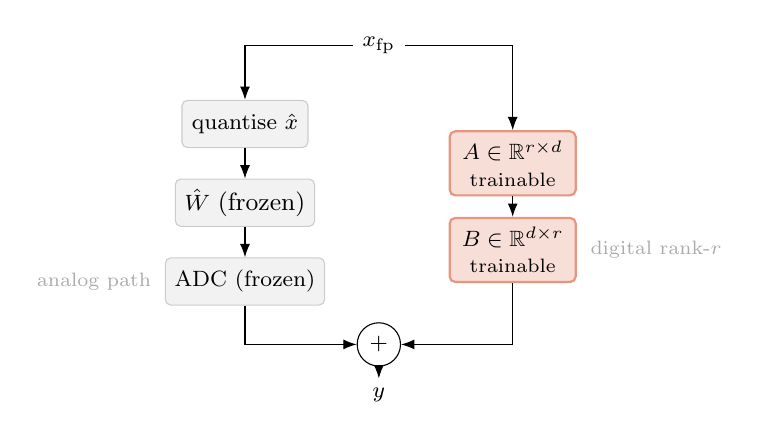
\begin{tikzpicture}[
    every node/.style={font=\footnotesize},
    box/.style={draw, rounded corners=2pt, minimum width=1.6cm, minimum height=0.6cm, align=center},
    frozen/.style={fill=mygray!15, draw=mygray!60},
    traina/.style={fill=myorange!25, draw=myorange!80, thick},
    sum/.style={draw, circle, minimum size=0.55cm, inner sep=0pt},
    lab/.style={font=\scriptsize, text=mygray}
  ]
  \node (x) at (0, 3.5) {$x_{\mathrm{fp}}$};
  \node[box, frozen] (qx) at (-1.7, 2.5) {quantise $\hat x$};
  \node[box, frozen] (w)  at (-1.7, 1.5) {$\hat W$ \small(frozen)};
  \node[box, frozen] (adc) at (-1.7, 0.5) {ADC (frozen)};
  \draw[-{Latex}] (x) -| (qx);
  \draw[-{Latex}] (qx) -- (w);
  \draw[-{Latex}] (w) -- (adc);
  \node[box, traina] (a) at (1.7, 2.0) {$A\in\mathbb R^{r\times d}$\\ \scriptsize trainable};
  \node[box, traina] (b) at (1.7, 0.9) {$B\in\mathbb R^{d\times r}$\\ \scriptsize trainable};
  \draw[-{Latex}] (x) -| (a);
  \draw[-{Latex}] (a) -- (b);
  \node[sum] (plus) at (0, -0.3) {$+$};
  \draw[-{Latex}] (adc.south) |- (plus);
  \draw[-{Latex}] (b.south) |- (plus);
  \node[below=0.15cm of plus] (y) {$y$};
  \draw[-{Latex}] (plus) -- (y);
  \node[lab, left=0.05cm of adc.west] {analog path};
  \node[lab, right=0.05cm of b.east] {digital rank-$r$};
\end{tikzpicture}}
\caption{Post-ADC residual LoRA (Phase 2). The quantized analog path (weights, transforms, diagonals, and ADC) stays frozen; a trainable rank-$r$ branch $B(A\,x_{\mathrm{fp}})$ is added \emph{after} the ADC in the digital domain, correcting the residual error the fixed lattice cannot express.}
\label{fig:lora}
\end{figure}

Even the best staged checkpoint leaves an ADC gap, and this ceiling is structural: pure PTQ can only reshape the signal \emph{before} the ADC. Once the converter maps a continuous accumulation to a discrete code, all sub-step information inside that bin is gone from the frozen analog path---which is why pure PTQ plateaus around $27.5$--$28.5$ W4A4 ADC perplexity across calibration strategies. Phase~2 therefore adds a small digital residual branch \emph{after} the ADC (Figure~\ref{fig:lora}). For a projection with frozen ADC output, the adapted output is
\begin{equation}
    y = \mathrm{ADC}_{\mathrm{frozen}}(\hat{x}) + \frac{s}{r}\,B\!\left(A\,x_{\mathrm{fp}}\right),
    \label{eq:lora}
\end{equation}
with $A \in \mathbb{R}^{r\times d}$, $B \in \mathbb{R}^{d_{\mathrm{out}}\times r}$, rank $r = 4$, and LoRA scale $s = 8$, computed in float32 (we reserve $\alpha$ for the calibration mixing coefficient). The entire base---weights, Kronecker factors, diagonals, and ADC steps---stays frozen. Rank-4 adapters on all seven projections of Llama-3.2-1B add ${\approx}2.8$M parameters ($0.23\%$ of the model); per-model counts are listed in Appendix~A of the supplementary material. The adapters are trained with next-token cross-entropy plus teacher distillation,
\begin{equation}
    \mathcal{L}_{\mathrm{LoRA}} = \mathrm{CE}(\hat{p}, y) + \lambda\,\mathrm{KL}\!\left(\hat{p}_T \,\|\, p_{\mathrm{FP},T}\right),
    \label{eq:lora_loss}
\end{equation}
with $\lambda = 0.5$ and temperature $T = 2$. Post-ADC placement is essential: a pre-ADC adapter is itself quantized by the fixed lattice, cannot express sub-$\Delta$ corrections, and diverges (ADC perplexity $\approx 105.6$). Post-ADC, the correction is added in the digital domain at full precision with clean gradients, dropping W4A4 ADC perplexity from $27.60$ to $14.03$.

\section{Experiments}

\subsection{Setup}

\paragraph{Models.}
We evaluate four sub-2B open-weight decoder-only LLMs: Llama-3.2-1B \citep{dubey2024llama} ($16$ layers, hidden size $2048$, grouped-query attention, SwiGLU FFN of width $8192$), Qwen2.5-1.5B \citep{qwen2025qwen25}, OLMo-1B \citep{groeneveld2024olmo}, and TinyLlama-1.1B \citep{zhang2024tinyllama}. TinyLlama shares the Llama architecture; Qwen2.5 and OLMo expose the same seven linear projections per decoder block, to which the per-projection transform wrappers were adapted. The models are small enough to sweep dozens of configurations on a single GPU while covering distinct pretraining corpora and tokenizers.
% NOTE(code): before trusting Qwen2.5/OLMo numbers, verify that the adapted FlatQuant
% wrappers are used -- ADC/llama/core/flat_quant.py wraps Llama-specific classes
% (apply_flatquant_to_model, lines 985-991; strip rebuilds LlamaMLP at line 1047).

\paragraph{Data and metrics.}
Calibration and LoRA training use WikiText-2 training text \citep{merity2017pointer} ($1024$ calibration samples; static activation scales from $99.9$th-percentile clipping). We report WikiText-2 and C4 \citep{raffel2020exploring} perplexity with context length $2048$ and stride $1024$, and downstream accuracy via lm-evaluation-harness \citep{gao2024lmeval} on eight tasks: HellaSwag \citep{zellers2019hellaswag}, MMLU \citep{hendrycks2021mmlu}, WinoGrande \citep{sakaguchi2021winogrande}, ARC-Easy/Challenge \citep{clark2018arc}, PIQA \citep{bisk2020piqa}, OpenBookQA \citep{mihaylov2018openbookqa}, and BoolQ \citep{clark2019boolq}.

\paragraph{Hardware setting and protocol.}
The main signed readout uses tile size $M = 256$, ADC bit-width $b_a = 8$, scaling factor $k = 16$, and W4A4 or W8A8 precision, giving $\Delta \approx 2016$ for W8A8 and $\Delta \approx 6.12$ for W4A4 (Eq.~\ref{eq:delta}). We report two perplexities: \emph{bypass} disables the ADC and isolates tiling plus integer quantization, while \emph{ADC} enables the full pipeline and is the primary metric; their gap measures ADC-induced degradation. Internal diagnostics (dead-rate, clip-rate, bin usage, reconstruction error) are defined in Appendix~A of the supplementary material. FlatQuant transforms train for $30$ epochs at $5\times10^{-3}$ (Stage~B: $10$ epochs at $5\times10^{-4}$); post-ADC LoRA trains for $5$ epochs at $10^{-4}$.

\subsection{Main Results}

\begin{table*}[t]
\centering
\small
\setlength{\tabcolsep}{5pt}
\begin{tabular}{@{}l rr rr rr rr@{}}
\toprule
& \multicolumn{2}{c}{Llama-3.2-1B} & \multicolumn{2}{c}{Qwen2.5-1.5B} & \multicolumn{2}{c}{OLMo-1B} & \multicolumn{2}{c}{TinyLlama-1.1B} \\
\cmidrule(lr){2-3}\cmidrule(lr){4-5}\cmidrule(lr){6-7}\cmidrule(lr){8-9}
Method & Wiki & C4 & Wiki & C4 & Wiki & C4 & Wiki & C4 \\
\midrule
BF16                        & 8.68    & 13.13 & \phnum & \phnum & \phnum & \phnum & 7.01 & 10.72 \\ % TODO(qwen25_15b,olmo_1b): fp rows
INT8 PTQ (ADC off)          & 8.69    & 13.15 & \phnum & \phnum & \phnum & \phnum & \phnum & \phnum \\ % TODO(qwen25_15b,olmo_1b,tinyllama_11b): int8 bypass
INT8 + ADC PTQ              & 16.85   & 29.56 & \phnum & \phnum & \phnum & \phnum & \phnum & \phnum \\ % TODO(qwen25_15b,olmo_1b,tinyllama_11b): int8 adc
INT4 PTQ (ADC off)          & 14.13   & 22.83 & \phnum & \phnum & \phnum & \phnum & \phnum & \phnum \\ % TODO(qwen25_15b,olmo_1b,tinyllama_11b): int4 bypass
INT4 + ADC, naive PTQ       & 2354.86 & ---   & \phnum & \phnum & \phnum & \phnum & \phnum & \phnum \\ % TODO(qwen25_15b,olmo_1b,tinyllama_11b): naive collapse
INT4 + ADC PTQ (ours)       & 26.66   & 45.62 & \phnum & \phnum & \phnum & \phnum & 11.62 & 20.23 \\ % TODO(qwen25_15b,olmo_1b): phase-1 result
INT4 + ADC + LoRA (ours)    & \textbf{14.03} & \textbf{23.20} & \phnum & \phnum & \phnum & \phnum & \phnum & \phnum \\ % TODO(qwen25_15b,olmo_1b,tinyllama_11b): phase-2 result
\bottomrule
\end{tabular}
\caption{Main results: WikiText-2 and C4 perplexity (lower is better) under the signed readout, single unified recipe per model. ``ADC off'' rows use tiled integer quantization with the ADC bypassed; ``+ ADC'' rows enable the full analog path. \phnum{}: runs in progress. The naive-PTQ row uses standard FlatQuant calibration with the ADC enabled at evaluation only.}
\label{tab:main}
\end{table*}

\begin{table}[t]
\centering
\small
\setlength{\tabcolsep}{4pt}
\begin{tabular}{@{}l rrrr@{}}
\toprule
Method & Llama & Qwen2.5 & OLMo & TinyLl. \\
\midrule
BF16                     & 54.25 & \phnum & \phnum & 44.08 \\ % TODO(qwen25_15b,olmo_1b): downstream avg
INT4 PTQ (ADC off)       & 48.64 & \phnum & \phnum & \phnum \\ % TODO(models): downstream avg
INT4 + ADC PTQ           & 41.99 & \phnum & \phnum & 41.81 \\ % TODO(qwen25_15b,olmo_1b): downstream avg
INT4 + ADC + LoRA        & \textbf{47.07} & \phnum & \phnum & \phnum \\ % TODO(models): downstream avg
\bottomrule
\end{tabular}
\caption{Average accuracy over the eight downstream tasks (higher is better). Per-task breakdowns for each model are in Appendix~F of the supplementary material.}
\label{tab:downstream_avg}
\end{table}

Table~\ref{tab:main} reports perplexity for all four models under a single unified recipe per model, and Table~\ref{tab:downstream_avg} the average downstream accuracy. We quote Llama-3.2-1B numbers in the text; cross-model statements refer to Table~\ref{tab:main}.
% TODO(models): once the qwen25_15b/olmo_1b/tinyllama_11b runs land, add 1-2 sentences here
% on cross-model consistency (does the naive collapse / recovery / LoRA ranking replicate?)
% and call out any model that deviates.

Digital PTQ and ADC-enabled PTQ are qualitatively different settings. At INT8, digital quantization is essentially lossless---WikiText-2 moves from $8.68$ to $8.69$---yet enabling the ADC degrades the same checkpoint to $16.85$ (C4: $29.56$), and the downstream average drops from $55.95$ to $44.97$. The pattern is stronger at INT4: the digital baseline remains usable ($14.13$/$22.83$), while the ADC-enabled model reaches only $26.66$/$45.62$ \emph{after} ADC-aware calibration---a conservative comparison, since that row is already calibrated for the ADC. Without ADC-aware calibration the naive W4A4 baseline collapses to $2354.86$; Phase~1 recovers a factor of ${\approx}88$, but remains ${\approx}3.1\times$ above the BF16 reference. Transform-based PTQ thus turns a collapsed model into a usable one, yet it cannot cross the hardware-defined floor: it acts strictly before the fixed lattice.

Phase~2 closes most of the remaining gap. Post-ADC LoRA reduces WikiText-2/C4 ADC perplexity from $26.66/45.62$ to $14.03/23.20$, closing ${\approx}70\%$ of the WikiText-2 and ${\approx}69\%$ of the C4 gap to BF16. The C4 result matters doubly: the adapter is trained on WikiText-2 only, so the improvement on held-out C4 indicates a systematic correction of ADC-distorted representations rather than memorization of the calibration text. Downstream accuracy improves from $41.99$ to $47.07$, recovering ${\approx}76\%$ of the ADC-induced drop relative to the digital INT4 reference; the largest gains appear on HellaSwag, ARC-Easy, PIQA, and OpenBookQA, while MMLU and WinoGrande improve less---expected, since the training signal is next-token CE+KL rather than task-specific.

One comparison deserves honest framing. INT4 + ADC + LoRA does not outperform the ideal \emph{digital} INT8 PTQ baseline, which is a no-ADC, near-full-precision reference. The relevant analog comparison is INT8 + ADC PTQ---and against it, INT4 + ADC + LoRA achieves lower perplexity on both corpora ($14.03$ vs.\ $16.85$; $23.20$ vs.\ $29.56$) and higher downstream accuracy ($47.07$ vs.\ $44.97$) despite using 4-bit codes in the analog path. Post-ADC correction thus makes a 4-bit ADC-enabled path competitive with, and here stronger than, an 8-bit ADC-enabled PTQ baseline.

\subsection{Ablation Summary}

Table~\ref{tab:ablation} condenses the ablations that justify each design choice; full tables and plots are in Appendices~C--D of the supplementary material. Three findings deserve emphasis. First, propagation is the single dominant calibration lever, and the mixed $\alpha=0.5$ objective is what makes it usable at INT4. Second, calibration data matters: moving from $128$ to $512$ samples with propagation collapses the bypass--ADC gap from $\times153$ to $\times1.2$. Third, all LoRA configurations push ADC perplexity \emph{below} bypass (gap $<1$), confirming that the adapter specifically corrects ADC-induced error rather than generically improving the digital path.

\begin{table}[t]
\centering
\footnotesize
\setlength{\tabcolsep}{3pt}
\begin{tabular}{@{}p{1.85cm}p{3.35cm}r@{}}
\toprule
Axis & Finding & ADC PPL \\
\midrule
Propagation (INT8) & propagation is the dominant lever & $28.86 \to 14.55$ \\
$\alpha$-mix (INT4) & $\alpha{=}0.5$ best; full prop.\ too noisy & $56.83 \to 27.56$ \\
Calib.\ samples & $128{\to}512$ closes $\times153 \to \times1.2$ gap & --- \\
Diag.\ placement & staged MLP${\to}$attn is best pure PTQ & $27.60$ \\
MLP decomp. & \texttt{down} diagonal drives the gain & --- \\
Stochastic $\alpha$ & no gain over deterministic $0.5$ & --- \\
LoRA rank & saturates at $r{=}4$ & --- \\
LoRA loss & CE+KL $\gg$ CE with all-7 targets & $16.68 \to 14.03$ \\
LoRA coverage & all 16 layers $\gg$ last 8 & $15.63$ vs.\ $20.08$ \\
LoRA placement & pre-ADC diverges & $14.03$ vs.\ $105.6$ \\
\bottomrule
\end{tabular}
\caption{Ablation summary (Llama-3.2-1B, signed readout; ablations are single-model by design). Full tables: Appendices~C--D of the supplementary material.}
\label{tab:ablation}
\end{table}

\subsection{Unsigned Shift-Subtract Readout}

The signed readout is a useful reference, but many physical crossbars accept only non-negative excitations. We therefore evaluate an unsigned shift-subtract readout on Llama-3.2-1B: signed INT4 codes are shifted to $[0,15]$, a single non-negative MVM is performed, and deterministic zero-point terms are subtracted digitally after ADC readout (exact recovery; derivation in Appendix~E of the supplementary material). The unsigned step at global $k = 16$ is $\Delta_u \approx 14.06$ (Eq.~\ref{eq:delta_u}), more than twice the signed W4A4 step. Because this coarser step imposes a heavier resolution penalty, we add a per-layer search over $k \in \{4,8,16,32,64\}$: for each projection, the search selects the smallest $k$ that avoids ADC saturation on the calibration set, running in place on the frozen PTQ checkpoint.

Table~\ref{tab:unsigned} shows that the global unsigned baseline ($39.00$) is much worse than the signed reference. Per-layer $k$ search alone reduces it to $21.64$ without retraining; post-ADC LoRA reaches $17.29$; their combination reaches $14.56$. Range adaptation before deployment and residual correction after the ADC are complementary, and both transfer to the more hardware-realistic unsigned readout.

\begin{table}[t]
\centering
\small
\setlength{\tabcolsep}{4pt}
\begin{tabular}{@{}l|cc@{}}
\toprule
Unsigned configuration & Wiki PPL & C4 PPL \\
\midrule
BF16 & 8.68 & 13.13 \\
INT4 FlatQuant, ADC off & 12.56 & 20.13 \\
Unsigned PTQ, global $k=16$ & 39.00 & 67.78 \\
\quad + per-layer $k$ & 21.64 & 33.79 \\
\quad + post-ADC LoRA & 17.29 & 29.26 \\
\quad + per-layer $k$ + LoRA & \textbf{14.56} & \textbf{23.78} \\
\bottomrule
\end{tabular}
\caption{Unsigned shift-subtract readout on Llama-3.2-1B. Per-layer $k$ search and post-ADC LoRA are complementary.}
\label{tab:unsigned}
\end{table}

\section{Discussion}

\paragraph{ADC error is not digital quantization error.}
Ordinary low-bit PTQ quality does not predict analog deployment quality. The ADC is applied after accumulation, where information from many channels has already been mixed into one value; if two distinct accumulations round to the same code, no downstream computation can separate them again. A model can therefore look healthy under no-ADC evaluation and fail once the converter is enabled. Bypass perplexity is a useful diagnostic for separating the two error sources, but never a deployment criterion: the ADC must be evaluated inside the inference loop.

\paragraph{ADC-aware calibration is distribution matching.}
Clean teacher activations do not match what deeper blocks receive at analog deployment time, where every input has already passed through many ADC readouts. Cross-block propagation does not add capacity; it makes the calibration signal faithful to the deployment signal, so error accumulation becomes visible during PTQ. Matching deployment too aggressively is harmful, however: ADC-propagated inputs carry noisy, non-smooth gradients, especially at INT4. The mixed objective is the resulting trade-off---enough clean signal to learn useful transforms, enough ADC signal to avoid overfitting an idealized digital path.

\paragraph{Outliers turn the ADC into a range-allocation problem.}
A few channels dominate activation magnitude but cannot simply be clipped away, so the converter must split its finite range between preserving outliers and resolving the bulk. This reframes rotations and diagonals as range-allocation tools: rotations spread energy across channels, and diagonals add the per-channel control that Lemma~\ref{lem:rotation} shows rotations cannot provide. The ablations sharpen the picture: MLP-side scaling mainly improves the low-bit transform itself, while attention-side scaling drives robustness to ADC noise---which is exactly why the staged schedule, separating the two problems, beats joint training.

\paragraph{Why pure PTQ has a ceiling, and why post-ADC correction crosses it.}
The PTQ plateau is not an optimization artifact. Every FlatQuant-style transform acts before the converter; once the ADC selects an output code, all sub-$\Delta$ variation inside that bin is removed from the frozen analog path, and no pre-ADC reshaping can represent a correction that must be applied after the code was chosen. A post-ADC branch is qualitatively different from one more pre-ADC transform: it operates on the digital side of the boundary, at full precision, with clean gradients. The held-out C4 improvement supports this reading---the adapter learns a systematic compensation for ADC-distorted representations, not the calibration text.

\paragraph{Hardware--software co-design.}
Changing the readout (signed vs.\ unsigned, range scaling $k$, tile width) changes the effective lattice and therefore the calibration problem itself: the same recipe that yields $26.66$ under the signed readout starts from $39.00$ under the coarser unsigned step. Modest hardware configurability is disproportionately valuable when exposed to calibration---per-layer $k$ alone recovers $39.00 \to 21.64$ with no retraining. Practical guidelines follow: evaluate ADC-on end to end; calibrate on the signal path the hardware will actually produce; treat outliers as an ADC-range problem; and prefer a small digital correction over full hardware-aware retraining when the budget is post-training only.

\section{Limitations}

All experiments use a software ADC simulator; real devices add non-uniform bins, offset, drift, thermal noise, IR drop, and latency constraints that the simulator deliberately abstracts, so hardware validation remains necessary. The evaluation covers four sub-2B models---larger models may show different outlier statistics and calibration budgets. Adaptation data is WikiText-2 with C4 as transfer evidence; broader deployment domains may shift activation distributions and the optimal transforms. The ADC model is a uniform fixed-step lattice; per-layer $k$ explores only one form of hardware configurability. Finally, the post-ADC branch has nonzero digital overhead and needs access to the adapter input; an accelerator design must decide whether it runs on a digital co-processor, is restricted to selected projections, or is fused into other post-processing.

\section{Conclusion}

We asked whether a pretrained LLM can be adapted to a fixed, finite-resolution ADC without retraining, and answered the five questions posed earlier. \textbf{RQ1:} the ADC is a dominant error source, not a detail---digital W8A8 is lossless ($8.69$) while the same checkpoint under the ADC reaches $16.85$, and the naive INT4 baseline collapses to $2354.86$. \textbf{RQ2:} transform-based PTQ recovers a factor of ${\approx}88$ of that collapse ($\to 26.66$) but plateaus ${\approx}3.1\times$ above BF16---a hardware-defined floor. \textbf{RQ3:} explicitly ADC-aware objectives are required: propagation halves INT8 ADC perplexity, and $\alpha = 0.5$ beats both clean and fully propagated calibration at INT4. \textbf{RQ4:} sensitivity is heterogeneous and exploitable---MLP and attention diagonals play different roles, and per-layer $k$ search alone recovers $39.00 \to 21.64$ on the unsigned readout. \textbf{RQ5:} beyond the PTQ plateau, a rank-4 post-ADC residual correction with $0.23\%$ extra parameters reaches $14.03/23.20$ (WikiText-2/C4), surpassing the INT8 ADC baseline, while a pre-ADC twin diverges.

The broader message is that the analog--digital boundary is an algorithmic object. ADC-aware PTQ makes analog low-bit LLM inference usable; post-ADC digital correction is what moves it beyond the PTQ plateau. Treating the converter as part of the quantization pipeline---rather than as a passive hardware detail---is essential for making low-bit LLMs work on analog accelerators.

\bibliography{adc_aware_llm_article_refs}

\end{document}
